General purpose {\em Succinct Non-interactive Arguments of Knowledge} (SNARKs) enable one to generate succinct
proofs of membership of a statement in an $\npol$ relation expressed as an arithmetic circuit. These proofs are
extremely cheap to verify, which makes them useful for {\em Verifiable Computation} (VC), where a resource-constrained
client (e.g., a mobile phone), can outsource an expensive computation to an untrusted server, and later
verify the correctness of the computation at a minimal cost.

\smallskip

\noindent{\bf Modeling RAM in Verifiable Computation.} It turns out that arithmetic circuit-based representations are inefficient in expressing relations involving the result of a program execution on memory/state. Such relations frequently arise in the context of verifiable computation, in scenarios that require proving the correctness of query execution against a database, inference from a decision tree, or updates on a table of account balances~(e.g., when a batch of transactions, such as account transfers, is applied to the table).

In the aforementioned examples, objects such as database tables, decision trees, and accounts tables can be naturally
modelled as instances of addressable memory, or more generally, random access memory~(RAM), where one needs to prove that the RAM has been accessed/updated in accordance with the correct execution of the computation. There exists a rich and expanding body of work on efficiently modeling abstractions of RAM in in verifiable computation. While a complete treatment of this vast body of work is beyond
the scope of this paper (a fairly recent survey in \cite{WB15} is a good starting point), we mention two additional properties that are often demanded of the RAM primitive: {\em persistence} -- the ability to persist the RAM state across several computations, and {\em batching} --
where verifiable update of the RAM state is required for small batches of updates. These properties are also the focus of this work.

%summarise key approaches towards
%modelling RAM in verifiable computation. Often we demand additional properties of the RAM primitive, such as
%{\em persistence} - which is the ability to persist the RAM state across several computations, and {\em batching} -
%where verifiable update of the RAM state is required for small batches of updates. 

\smallskip

\noindent{\bf Application to Blockchain Rollups.} Batching-efficient RAM is especially relevant in the context of blockchain {\em rollups} ~\cite{rollup},
an umbrella term for recent efforts to scale blockchains by moving expensive computation off the blockchain to the so-called {\em layer two}~(or L2) chains. The blockchain only needs to verify succinct proofs attesting to the correctness of the off-chain computation. This approach is popularly called \textit{rollup} as it allows verifying the result of several (rolled-up) transactions modifying the L2 state, as part of one transaction verified on the main chain.
This simultaneously improves scalability and lowers the cost (e.g., gas fees) per transaction due to succinct verification. We consider improving efficiency of rollups an important motivation for our work, but avoid precise details of a smart-contract based
instantiation of our solution.

\subsection{Our Contribution}\label{subsec:ourwork} 
We present batching-efficient RAM construction, which advances the efforts
towards achieving {\em verifiable outsourcing of state update} such as in ~\cite{EPRINT:BFRSBW13}
and more recently in ~\cite{USENIX:OWWB20, CCS:CFHKKO22}.
The most popular approaches to succinctly represent
state involve accumulators based on Merkle-trees ~\cite{C:Merkle87}, or ones based on groups of unknown order
(e.g. RSA, class-groups) ~\cite{C:CamLys02,C:BonBunFis19,USENIX:OWWB20, CCS:CFHKKO22}.
The updates to the state are effected by insertions or deletions in the  accumulated set.
In this work, we
model the state as an addressable memory (RAM) described by vector $\vecT$, which stores values $v_i$ at addresses $i$.
We denote this as $\vecT[\,i\,]=v_i$. The RAM supports two operations, viz, {\em loads} expressed
as $v_i := \vecT[\,i\,]$, and {\em stores} expressed as $\vecT[\,i\,]=v_i$.
%denoted by the tuple $(\load, i, v_i)$ and (ii) {\em indexed update} ($\vecT[\,i\,] := v_i$), denoted
%by the tuple $(\store, i, v_i)$.
We think of addresses $i\in [0,N]$ for some $N\in \mathbb{Z}$ while the
values $v_i\in \F$ for some finite field $\F$. In our construction, we represent both the RAM and operations on it
as polynomials, and use appropriate polynomial commitment schemes to obtain succinct commitments (digests) to them.
In this paper, we do not require commitments to be {\em hiding}, as our focus is on succinctness.
We consider privacy as an orthogonal goal, one we believe is easily achievable
via small adaptations to our construction.\smallskip


\begin{comment}
\noindent{\bf Application to Blockchain Rollups}: We consider the application of persistent RAM primitive to a common rollup scenario.
Our application is a simplified adaptation of rollup protocols such as ZkSync ~\cite{ZkSync}.
We assume a layer two (L2) chain \textsf{DemoChain}, which issues its clients \textsf{DemoCoins}. The clients have accounts on
L2, and they transfer \textsf{DemoCoins} to each other using L2 transactions. Such a system will also have mechanism to transfer
funds to and from main-chain (e.g. Ethereum) accounts, but we
ignore those details here.
Each client is assigned a unique identifier $i$, and associated account information  is maintained as
a tuple $(\pk_i,\bal_i,\txno_i)$ which refer respectively to the public key for verifying client's signature on transactions,
account balance (number of coins owned by the client) and total number of transactions made from the account (to prevent replay attacks).
The L2 state thus consists of the above information for all accounts. We model an L2 chain supporting upto $N$ accounts as a RAM $\vecT$
of size $N$, where $\vecT[\,i\,]=(\pk_i,\bal_i,\txno_i)$ denotes client $i$'s account information. A transfer transaction of amount $v$
from client $i$ to client $j$ involves two load operations, and two store operations on the RAM (for reading and updating the referenced
accounts). These transactions are submitted by clients directly to a designated L2 chain operator \textsf{DemoOperator}, who batches $m$
such transactions and updates the RAM state accordingly. The operator maintains the entire state off-chain and locally computes the updates for
each batch of transactions. Only the succinct digest of the state (polynomial commitments) is stored on the main chain, and the proof of
validity of the state update is verified by a main-chain transaction. In later sections, we provide more details on the application and the
performance achieved when instantiated using our primitive.
\end{comment}

We summarize our contributions below.
\begin{itemize}[leftmargin=2em]
	\item As our first contribution, we propose {\em update friendly lookup arguments}, which addresses
	the strict dependence of recent constructions on table-specific pre-processing parameters. Our
	innovation extends the utility of table-specific parameters to enable efficient lookups from tables,
	which are within certain hamming distance of the pre-processed table.
	\item We construct {\em committed index lookup} arguments via black-box reduction to
	sub-vector arguments that use homomorphic commitments. A committed index lookup involves
	three committed vectors $\vec{t},\vec{a}$ and $\vec{v}$ satisfying $v_i=t_{a_i}$ for all $i$. Similar
	definition is also used in recent multi-variate lookup arguments in ~\cite{lasso}, where a similar reduction
	to sub-vector arguments is obtained under a more restrictive assumption about the elements of the table.
	\item We crucially employ the above two contributions to construct a {\em batching-efficient} RAM, which
	can prove a batch of $m$ updates with an amortized prover complexity of $O(m\log m + \sqrt{mN})$,
	with $N$ being the size of the RAM. Our dependence on the RAM size is sub-linear, in contrast to the linear complexity
	inherent in recent works on batching-efficient RAM using RSA accumulators ~\cite{USENIX:OWWB20,CCS:CFHKKO22} or using generic memory checking techniques~\cite{NDSS:WSRBW15,USENIX:BCTV14,C:BCGTV13,SP:ZGKPP18}. All of our protocols are public-coin, and can be made non-interactive using standard techniques~\cite{C:FiaSha86}. 
	
	\item We implement our scheme in Rust\footnote{\url{https://anonymous.4open.science/r/updatableRAM/}}.
	Experimentally, we show that our scheme performs significantly better than prior works,
	and is eminently deployable on a commodity hardware.
\end{itemize}


\subsection{Techniques}\label{subsec:techniques}

We present a brief summary of our techniques below. A more detailed technical overview appears in Section~\ref{sec:tech-overview}.

\smallskip

\noindent{\bf Update-friendly Lookup Arguments.} Our starting point is the recent line of works on lookup arguments which prove
that a vector of size $m$ appears as
a sub-vector in a large fixed vector (table) of size $N$ with succinct proof sizes and verification, but most notably
ensuring that prover runs in time sub-linear in the size of the table ($N$). The pioneering work ~\cite{CCS:ZBKMNS22}
obtained prover complexity of $O(m^2+m\log N)$, which was improved in subsequent works to $O(m^2)$ ~\cite{EPRINT:PosKat22},
$O(m\log^2 m)$ ~\cite{EPRINT:ZGKMR22}, and $O(m\log m)$ ~\cite{EPRINT:EagFioGab22,PKC:CFFLL24}. However, the sub-linear prover
complexity requires table-dependent $O(N\log N)$ pre-processing and $O(N)$ storage. This table-dependent
pre-processing implies that while
the aforementioned lookup arguments can be used to obtain efficient ROM (read only memory) semantics
%\footnote{The protocols for sub-vector relation in ~\cite{CCS:ZBKMNS22, EPRINT:ZGKMR22} also implicitly support indexed lookup semantics},
they cannot be used as is for RAM (which supports update operations).
Moreover, an update involving even a single
index renders the entire $O(N)$ pre-processing unusable for further lookups,
thus necessitating entire $O(N\log N)$ re-computation. This work is the first effort towards
mitigating this rigid dependence, thereby increasing the applicability of the recent lookup arguments.
An important contribution we make here is a new method for computing ``encoded quotients'' used in several
recent lookup constructions such as~\cite{CCS:ZBKMNS22,EPRINT:PosKat22,EPRINT:EagFioGab22,PKC:CFFLL24}.
Our approach for computing these quotients from pre-computed parameters remains efficient even when
the table is updated, and it directly applies to all the aforementioned constructions.
For a table $\delta$-hamming distance away from the pre-processed one, we incur
$(m+\delta)\log^2(m+\delta)$ additional overhead for proving $m$ lookups. To achieve such a quasi-linear overhead in both $m$ and $\delta$, we rely on novel algebraic algorithms described in Section~\ref{sec:update-protocol}.
We informally summarize our contribution in this regard below, whereas Theorem~\ref{thm:approx-setup}
states the precise result.
\begin{theorem}[Informal]\label{thm:pre-process}
	There exists a deterministic $O(N\log N)$ time algorithm $\textsf{Preprocess}(\vecT)\outp \pp_T$
	which on input $\vecT\in \F^N$, outputs parameters $\pp_T$ of size $O(N)$ such
	that: Given $\pp_T$, vectors $\vecT'\in \F^N$, $\vec{t}\in \F^m$ with $\vec{t}$ being a sub-vector of $\vecT'$
	an argument of knowledge for the same can be computed in time
	$O((m+\delta)\log^2 (m+\delta) + f(m))$ where $\delta=\Delta(\vecT, \vecT')$
	is the hamming distance of $\vecT$ and $\vecT'$ while $f(m)$ depends on the specific lookup protocol.
\end{theorem}
For the constructions based on~\cite{CCS:ZBKMNS22,EPRINT:PosKat22}, we set $f(m)=m^2$ in the above,
while for~\cite{EPRINT:EagFioGab22,PKC:CFFLL24}, we have $f(m)=m\log m$.

\smallskip

\noindent{\bf Committed Index Lookup}: We augment the sub-vector relation in prior lookup arguments which
considers whether each entry of a given vector appears in the target vector to one that also identifies
the precise positions where the given vector appears in the target vector. When this relation is checked
over commitments of the respective vectors; given vector, the target vector and the position vector, we call
it {\em committed index lookup}. The relation we consider is similar to the one considered in ~\cite{lasso}.
For lookup arguments with homomorphic commitment schemes, we show that committed index lookup can be obtained
using a sub-vector lookup argument (Lemma~\ref{lem:generic-transformation}, Section~\ref{subsec:committed-index-lookup}). Such a construction was
also considered in~\cite{lasso}, but under a more restrictive assumption on the size of the elements in the table being
within a certain bound. Lemma~\ref{lem:generic-transformation} yields a construction of committed index lookup that uses (a single instance of) the underlying sub-vector protocol in a black-box manner. This immediately implies
efficient constructions of arguments for committed index lookups from
~\cite{CCS:ZBKMNS22,EPRINT:PosKat22,EPRINT:ZGKMR22,EPRINT:EagFioGab22,PKC:CFFLL24}. In Appendix~\ref{app:committed-index-lookup}, we also present an explicit (non-black-box) adaptation of~\cite{EPRINT:PosKat22} to obtain a committed index lookup, which again incurs costs comparable to a single instance of the underlying sub-vector protocol.

\smallskip


\noindent{\bf Batching-Efficient RAM from Lookup Arguments.}
Memory checking methods based on {\em address ordered transcripts}
~\cite{NDSS:WSRBW15,USENIX:BCTV14,C:BCGTV13,SP:ZGKPP18}, which are popularly used in
efficient RAM abstractions, incur a cost linear in the size of the RAM. This is prohibitive for efficient batching. As a key idea in this work, we invoke committed index lookup on
the large RAMs, to verifiably extract smaller sub-RAMs, which correspond to indices actually involved in
the batch update. Then, we use the linear time memory-checking techniques to argue the consistency of these
smaller sub-RAMs. 

The idea needs to work through some more details, such as showing that the larger RAMs are identical
on positions not referenced by the batch of updates (considered in Section ~\ref{subsec:proximity-ram}).
The overall idea is illustrated in Figure ~\ref{fig:blueprint}. We also note that the extracted sub-RAMs can
have duplicate records, corresponding to multiple updates referencing the same RAM index; however, memory
checking methods can be easily adapted to handle such cases. Finally, we would still hit the ``rigidity'' of lookup arguments
in realizing this plan; once the table has changed, lookups are no longer efficient from it. To circumvent this,
we use our first contribution on extending the utility of table-specific parameters to defer parameter
re-computation optimally while still availing efficient lookups. More specifically, if we choose to
re-compute the full table-specific parameters after $k$ batches (of $m$ updates each),
the average cost per batch is $O(N\log N/k + mk\log^2(mk) + f(m))$. Here, $f(m)$ as earlier denotes complexity
of the non-updatable base protocol. Setting $k\approx \sqrt{N/m}$ yields the average cost of $m$ updates as $\wt{O}(f(m)+\sqrt{mN})$,
which scales sub-linearly with the size of the RAM.
While the preceding analysis considers the worst case,
in specific applications (such as account transactions, where few accounts contribute a large volume of transactions), it may be
possible to further delay the computation of table-specific parameters.
Thus we have:
\begin{theorem}[Informal]\label{thm:inc-ver-ram-informal}
	Given $m,N\in \mathbb{N}$, there exists an argument for verifiable RAM which proves updates of batch size $m$ on RAM of size $N$
	with amortized prover complexity of $\wt{O}(f(m) + \sqrt{mN})$.
\end{theorem}


\noindent{\bf Polynomial Protocol for RAM.} There are several ways to implement the ordered transcript based
memory consistency check on the smaller $O(m)$-sized RAMs, for example by expressing the same as an arithmetic
circuit. However, for completeness, we also present an argument for RAM as an
interactive {\em polynomial protocol} ~\cite{Gabizon2019PLONKPO}, which is then compiled into an argument of knowledge using the $\kzg$ ~\cite{AC:KatZavGol10}
commitment scheme in the algebraic group model (AGM) ~\cite{C:FucKilLos18}. This construction appears in
Appendix ~\ref{sec:poly-proto-ram-app}.
%\moumita{Making all references to Sections in Appendix, as Appendix B instead of Section B.}

\begin{comment}
Most of the efficient implementations of RAM in verifiable computation ~\cite{C:BCGTV13, NDSS:WSRBW15, SP:ZGKPP18}
rely on the {\em address-ordered transcript} to check that a sequence of $\load$s and $\store$s are {\em consistent} with some initial state
of the RAM. Using the tuple $(t,\op,\ind, v)$ to denote a RAM instruction with $t$ being the execution {\em timestamp}, $\op\in \{\load,\store\}$ being
the operation type, $\ind$ being the index referenced and $v$ denoting the value read/stored, a time ordered execution transcript $\mathsf{tr} = (\ins_1,\ldots,\ins_m)$ is a sequence
of instructions where $\ins_i=(t_i,\op_i,\ind_i, v_i)$ and $t_i < t_{i+1}$ for all $1\leq i<m$. The transcript $\mathsf{tr}$ is said to be consistent if
for every $\load$ instruction $\ins=(t,\load,\ind,v)$, the value $v$ is the same as that for the most recent $\store$ instruction, which references the same index
as $\ins$. This consistency can be efficiently checked by permuting the transcript $\mathsf{tr}$ to produce the sequence
$\mathsf{tr}^\ast=(\ins_1^\ast,\ldots,\ins_m^\ast)$ with $\ins_i^\ast=(t_i^\ast,\op_i^\ast,\ind_i^\ast,v_i^\ast)$ which is sorted by index, with
timestamp used to break the ties, i.e, $\ind_i^\ast\leq \ind_{i+1}^\ast$ and whenever $\ind_i^\ast=\ind_{i+1}^\ast$, we have $t_i^\ast < t_{i+1}^\ast$.
We call the resulting transcript $\mathsf{tr}^\ast$ as address ordered transcript. On such a transcript, the consistency is enforced simply by
checking that each $\load$ instruction involves the same value $v$ as the previous instruction, provided the referenced indices are the same.
The above approach is easily extended to verify that result of executing a sequence of operations $\{(\op_i,\ind_i,v_i)\}_{i=1}^m$ on
RAM $\vecT_0\in \F^n$ is $\vecT_1\in F^n$. In this case, we define a transcript $\mathsf{tr}=(\ins_1,\ldots,\ins_{2n+m})$ where the
first $n$ instructions $\ins_i,i\in [n]$ are defined as $\ins_i=(i,\store,i,\vecT_0[\,i\,])$, the next $m$ instructions are defined
as $\ins_{n+i},i\in [m]$ as $\ins_{n+i}=(n+i, \op_i, \ind_i, v_i)$ and the last $n$ instructions $\ins_{n+m+i}, i\in [n]$ as
$\ins_{n+m+i}=(n+m+i,\load,i,\vecT_1[\,i\,])$. The consistency of the transcript $\mathsf{tr}$ is checked via address ordering permutation as
described before. Intuitively, the first $n$ instructions in $\mathsf{tr}$ copy the initial contents of the RAM, the next $m$ instructions essentially
capture the sequence of RAM operations executed on the initial RAM, while the final $n$ instructions read out the entire contents of the RAM which
is expected to match the contents of $\vecT_1[\,i\,]$. We illustrate this approach in Figure \ref{fig:permutated-transcripts}. One of the contributions of this work is a polynomial protocol that proves that RAM state
$\vecT_1\in \F^n$ is obtained from RAM state $\vecT_0\in \F^n$ as a result of sequence of operations $\vec{\op}=\{(\op_i,\ind_i,v_i)\}_{i=1}^m$, where each
of the vectors $\vecT_0,\vecT_1$ and $\vec{\op}$ are represented via polynomials. Informally, we show:
\begin{theorem}[informal]\label{thm:pp-for-ram-informal}
For $m,n\in \mathbb{N}$, there exists a polynomial protocol to prove that sequence of operations $\vec{\op}=\{(\op_i,\ind_i,v_i)\}_{i=1}^m$ updates a
RAM state $\vecT_0\in \F^n$ to RAM state $\vecT_1\in \F^n$ with the prover-complexity of $\tilde{O}(m+n)$.
\end{theorem}
\end{comment}

%and ~\ref{fig:subtable-consistency}
%illustrate the overall idea for the first check with a concrete example.


\begin{comment}
\begin{figure}[t]
\begin{subfigure}{0.4\textwidth}
\centering
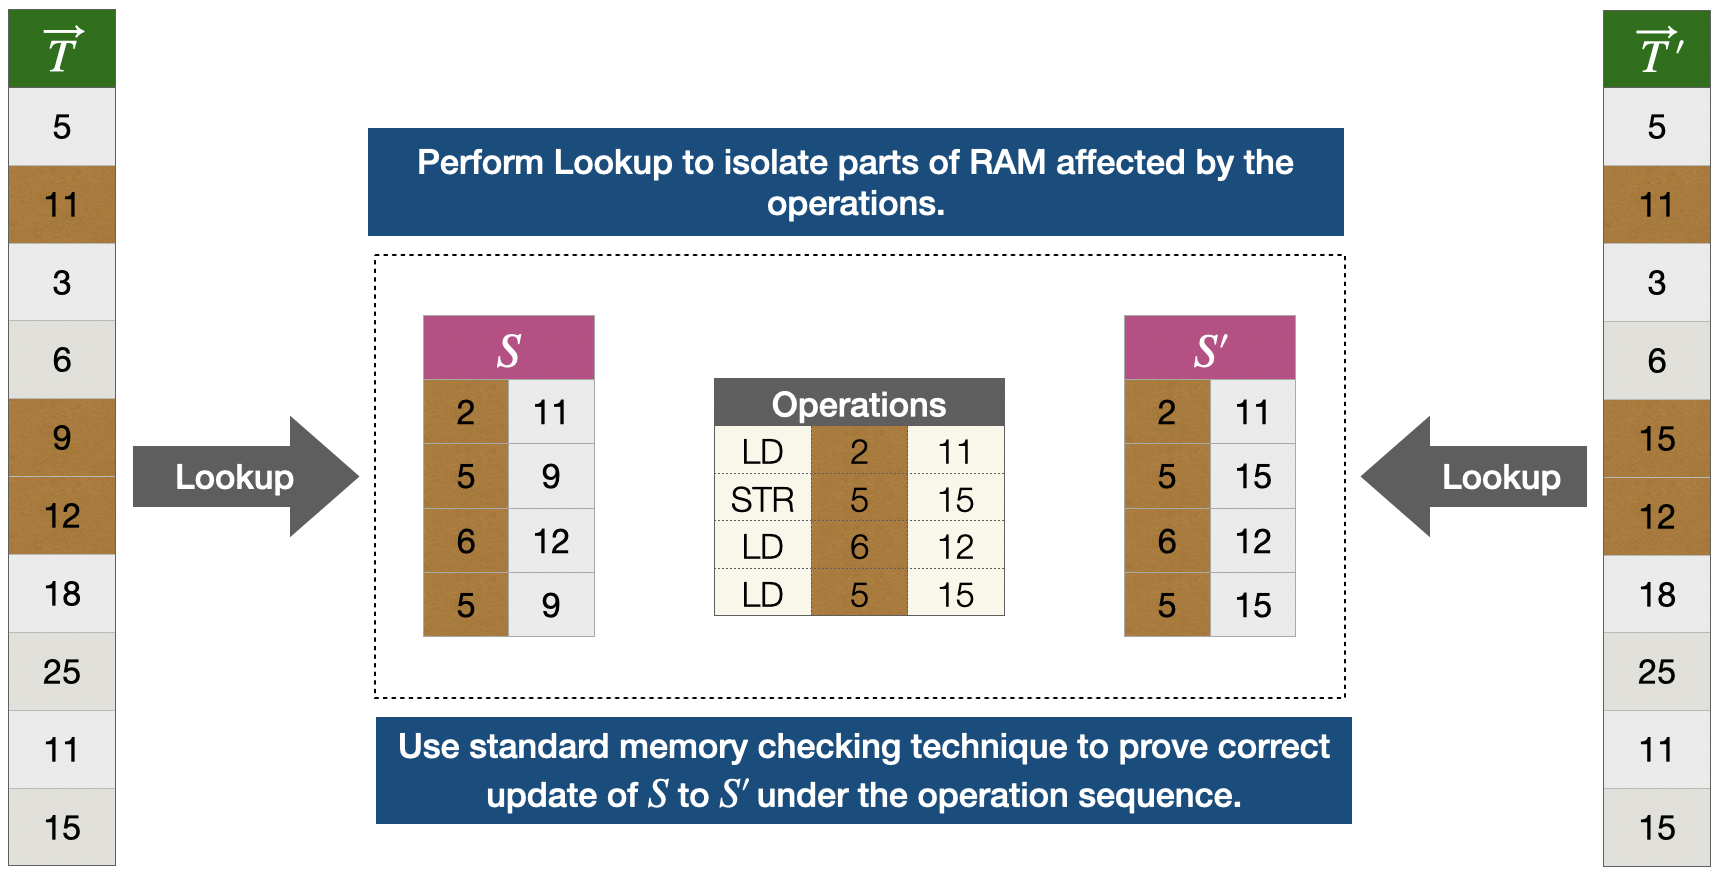
\includegraphics[width=\textwidth]{example-lookup}
\caption{Isolating subtables using lookup argument}
\label{fig:subtable-consistency}
\end{subfigure}
\begin{subfigure}{0.4\textwidth}
\centering
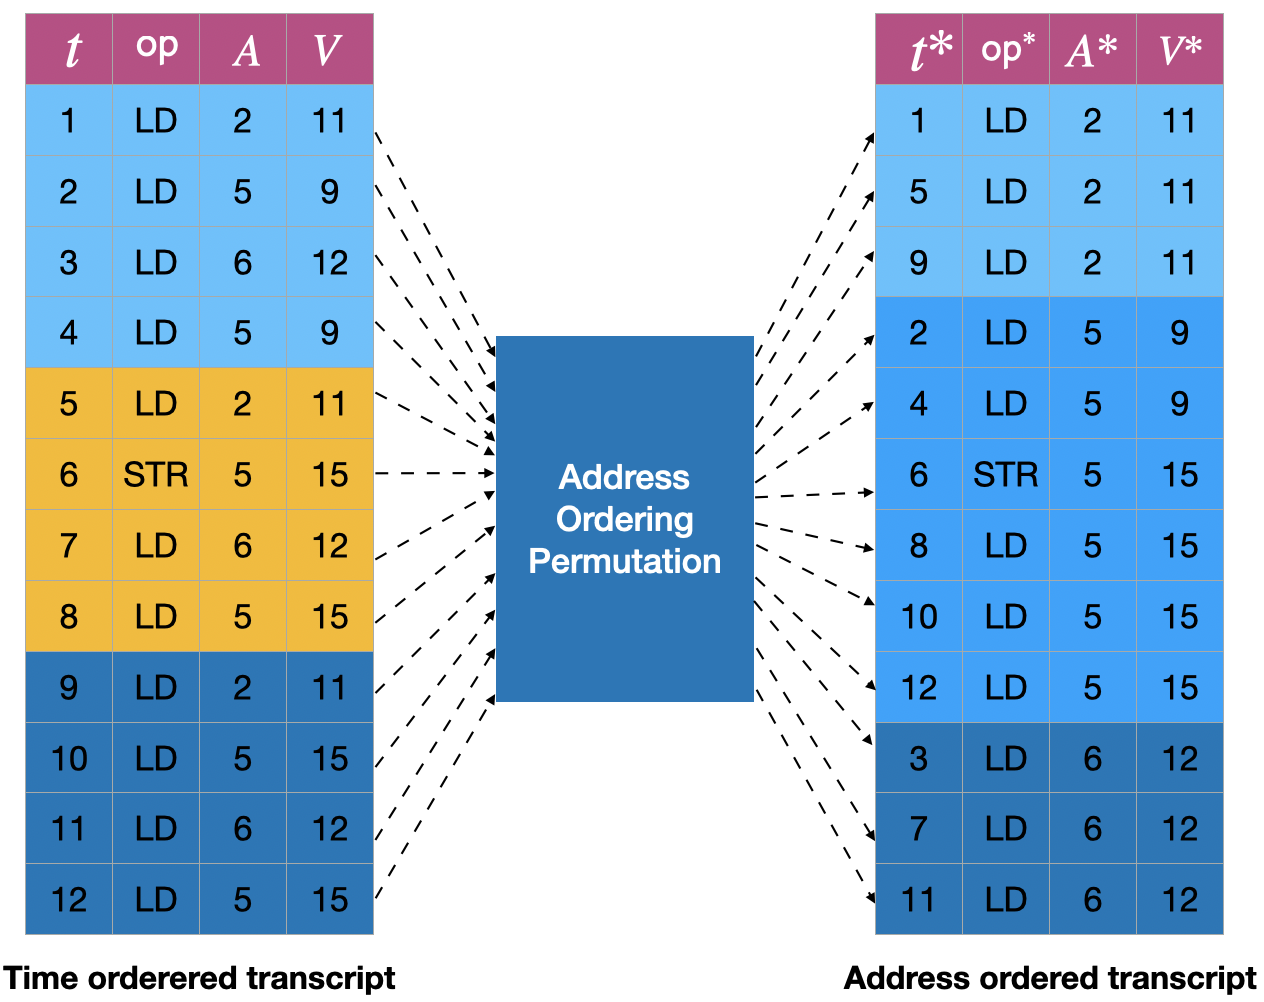
\includegraphics[height=0.3\textheight]{Address-ordered}
\caption{Checking memory consistency using address ordering}
\label{fig:permuted-transcripts}
\end{subfigure}
\end{figure}
\end{comment}



%
    \tikzset{
        table/.style={
            matrix of nodes,
            row sep=-\pgflinewidth,
            column sep=-\pgflinewidth,
            nodes={
                rectangle,
                draw=black,
                align=center
            },
            minimum height=1.5em,
            text depth=0.5ex,
            text height=1.5ex,
            nodes in empty cells,
%%
            every even row/.style={
                nodes={fill=gray!20}
            },
            column 1/.style={
                nodes={text width=2em}
            },
            row 1/.style={
                nodes={
                    fill=white,
                    text=black,
                    font=\bfseries
                },
            }
        }
    }

    \tikzset{
        MyArrow/.style={
            single arrow, draw=black, minimum width=10mm, minimum height=30mm, inner sep=0mm, single arrow head extend=1mm, double arrow head extend=1mm
        }
    }

    \begin{figure}[t]
        \centering
        %\subcaptionbox{Lookup to get sub-tables \label{fig:lookup}}[\textwidth]{
        \resizebox{0.8\textwidth}{0.3\textheight}{
        \begin{tikzpicture}
            %\draw[step=1.0,black,thin] (-5,-5) grid (5,5);
        \matrix (initial) [table,text width=2em, width=2cm] at (-5,1)
        {
            Idx & Val\\
            1  & 10 \\
            2  & 20 \\
            3  & 15 \\
            4  & 25 \\
            5  & 40 \\
            6 & 50 \\
            7 & 60 \\
        };

        \matrix (ops1) [table,text width=2em, width=2cm] at (0,0)
            {
            Op & Idx & Val \\
            \store  & 7 & 40 \\
            \load  & 1 & 10 \\
            \store & 3 & 20 \\
            \load  & 3 & 20 \\
        };


        \matrix (final) [table,text width=2em, width=2cm] at (5,1)
            {
            Idx & Val\\
            1  & 10 \\
            2  & 20 \\
            3  & 20 \\
            4  & 25 \\
            5  & 40 \\
            6 & 50 \\
            7 & 40 \\
        };


        % -------------------------------- Subtables ------------------------------------- %
        \matrix (stinitial) [table,text width=2em, width=2cm] at (-5,-5)
            {
            Idx & Val\\
            7 & 60 \\
            1 & 10 \\
            3 & 15 \\
            3 & 15 \\
        };

        \matrix (ops2) [table,text width=2em, width=2cm] at (0,-5)
            {
            Op & Idx & Val \\
            \store  & 7 & 40 \\
            \load  & 1 & 10 \\
            \store & 3 & 20 \\
            \load  & 3 & 20 \\
        };


        \matrix (stfinal) [table,text width=2em, width=2cm] at (5,-5)
            {
            Idx & Val\\
            7 & 40 \\
            1 & 10 \\
            3 & 20 \\
            3 & 20 \\
        };

            \draw (-5,3.6) node[above]  {\bf RAM $\vecT_0$};
            \draw (0, 1.6) node[above] {\bf Operations};
            \draw (5,3.6) node[above] {\bf RAM $\vecT_1$};
            \draw (-5, -3.4) node[above] {\bf $\vec{t}_0$};
            \draw (5, -3.4) node[above] {\bf $\vec{t}_1$};

            % lookup arrows
            \draw [-Latex, thick] (-4.25,-1.75) -- (-4.25,-3.25);
            \draw [-Latex, thick] (4.25, -1.75) -- (4.25, -3.25);
            \draw [fill=grey!30!white] (-2,-2) rectangle (2, -3) node[midway] {Lookup on indices 7,1,3,3};

            \draw (-2, -2.5) -- (-4.25, -2.5) (2, -2.5) -- (4.25, -2.5);
            \draw [-Latex, dashed] (-4, 0) -- (-1.6,0);
            \draw [-Latex, dashed] (1.6,0) -- (4,0);
            \draw [-Latex, dashed] (-4, -5) -- (-1.6,-5);
            \draw [-Latex, dashed] (1.6,-5) -- (4,-5);
        \end{tikzpicture}
        }
        \caption{Using lookup arguments to reduce the consistency check between large RAMs $\vecT_0$
        and $\vecT_1$ to that between small tables $\vec{t}_0$ and $\vec{t}_1$. It is seperately shown that RAMs $\vecT_0$ and
        $\vecT_1$ have identical values outside the involved indices. Figure ~\ref{fig:subtable-consistency} illustrates address
        ordered transcript to check consistency of $\vec{t}_0$ and $\vec{t}_1$.}
        \label{fig:subtable-lookup}
        \end{figure}

        \begin{figure}[htbp]
            \centering
            \resizebox{0.8\textwidth}{0.4\textheight}{
        \begin{tikzpicture}
        % ------------------------------------------------------------------------------------------- %
            %\draw[step=1.0,black,thin] (-5,-5) grid (5,5);
        \matrix (trts) [table,text width=2em] at (-4,0)
            {
            Ts & Op & Idx & Val\\
            1 & \store & 7 & 60 \\
            2 & \store & 1 & 10 \\
            3 & \store & 3 & 15 \\
            4 & \store & 3 & 15 \\
            5 & \store  & 7 & 40 \\
            6 & \load  & 1 & 10 \\
            7 & \store & 3 & 20 \\
            8 & \load  & 3 & 20 \\
            9 & \load & 7 & 40 \\
            10 & \load & 1 & 10 \\
            11 & \load & 3 & 20 \\
            12 & \load & 3 & 20 \\
        };

        \matrix (trts) [table,text width=2em, width=2cm] at (4,0)
            {
            Ts & Op & Idx & Val\\
            2 & \store & 1 & 10 \\
            6 & \load & 1 & 10 \\
            10 & \load & 1 & 10 \\
            3 & \store & 3 & 15 \\
            4 & \store  & 3 & 15 \\
            7 & \store  & 3 & 20 \\
            8 & \load & 3 & 20 \\
            11 & \load  & 3 & 20 \\
            12 & \load & 3 & 20 \\
            1 & \store & 7 & 60 \\
            5 & \store & 7 & 40 \\
            9 & \load & 7 & 40 \\
        };

            \path (-2.1,0) -- (1.9, 0)  node[midway, MyArrow, text width=3cm, align=center] {Address-sorting permutation};
            \draw (-4, 4.3) node[above] {\bf \small Time ordered transcript ($\mathsf{tr}$)};
            \draw (4, 4.3) node[above] {\bf \small Address ordered transcript ($\mathsf{tr}^\ast$)};

        \end{tikzpicture}
            }
            \caption{Address ordered transcript for checking consistency of tables $\vec{t}_0$ and $\vec{t}_1$
                with respect to the operation sequence in Figure \ref{fig:subtable-lookup}. On the transcript
            $\mathsf{tr}^\ast$, one checks that the load instructions return the same value as the preceeding
            instruction if their indices are the same.}

        \label{fig:subtable-consistency}
    \end{figure}

